\chapter{Probability space intro}
\section{probability space}
我们这里跳过所有 measure theory 的内容, 见 notes on measure theory.\\
\begin{definition}{prob space, prob measure, sample space, event space}
    一个 probability space 就是一个 measure space \( (\Omega, \mathcal{F}, \mathbb{P}) \), 其中 $\mathbb{P}(\emptyset) =0, \mathbb{P}(\Omega) = 1$.\\
    对于这样的 measure $\mathbb{P}$, 我们称之为 \textbf{probability measure (概率测度, 即概率)}.\\
    而这里的 \(\Omega\) 我们称之为 \textbf{sample space (样本空间)}; 这里的 $\sigma$-algebra $\mathcal{F}$, 我们称之为 \textbf{event space (事件空间)}. \\
    任意的 $A \subset \Omega$ 都是一个 \textbf{event}, 但是概率论中只考虑 $A\in\mathcal{F}$, 即 measurable event. 为简化, event 这个单词就指 measurable event.
\end{definition}
\begin{remark}
    回顾一下 measure space 的定义:
    \begin{itemize}
        \item 一个 set $\Omega$ 的一个 $\sigma$-algebra 就是一个包含空集的子集簇, 其 \textbf{closed under countable unions and complements}. (如果只 closed under finite unions, 则只称为一个 algebra.)
        \item 一个 Borel algebra 是一个定义在 topological space 上的 $\sigma$-algebra, 由 all open sets 生成. (因而: closed under countable unions and complements.) $\mathbb{R}$ 的 Borel algebra 可以由 all open intervals 生成.
        \item 一个 measure on a measurable space $(\Omega, \mathcal{F})$ 就是一个从 $\mathcal{F} \to \mathbb{R}$ 的函数, 满足 \textbf{countable additivity}.
        \item measure 的性质: \textbf{(1)non-negativity, (2) monotonicity, (3) countable subadditivity, (4) inclusion-exclusion principle (上节已讲), (5) continuity from below and above.} 第 (5) 条具体即:
        For measurable sets $A_1 \subseteq A_2 \subseteq \cdots \subseteq A_n \subseteq \cdots$, then $\lim_{n \to \infty} \mathbb{P}(A_n) = \mathbb{P}(\bigcup_{n=1}^{\infty} A_n)$.\\
        For measurable sets $A_1 \supseteq A_2 \supseteq \cdots \supseteq A_n \supseteq \cdots$, then $\lim_{n \to \infty} \mathbb{P}(A_n) = \mathbb{P}(\bigcap_{n=1}^{\infty} A_n)$.
    \end{itemize}
\end{remark}
\begin{remark}
    对于 discrete 的 prob space 而言, 通常选取 $\mathcal{F} = 2^{\Omega}$, 即 $\Omega$ 的任意子集都是一个 event.
\end{remark}
\begin{remark}
    概率空间的现实意义是: 一次 experiment 的所有可能的结果的集合, 以及每个结果的概率.
    \begin{align*}
        \Omega &= \{\omega \mid \omega \text{ 是一次 experiment 的可能的结果}\}\\
        \mathbb{P}(\omega) &= \text{ 结果 $\omega$ 的可能性}
    \end{align*}
\end{remark}

\begin{example}
    (dice roll) 
    如果我们掷一个 6 面的骰子, 那么样本空间 $\Omega=\{1,2,3,4,5,6\}$. 一个可能的事件是 $A=\{1,2\}$. 如果假设骰子是公平的 (所有结果都是等可能的), 那么事件 $A$ 的概率是
    \[
    \mathbb{P}(A)=\frac{\text { Number of favorable outcomes }}{\text { Total number of outcomes }}=\frac{|A|}{|\Omega|}=\frac{2}{6} 
    \]
    % 如果我们定义一个随机变量 $X$ 表示掷骰子的结果, 那么 $X$ 的样本空间是 $\mathbb{R}$, 即 $X: \Omega \rightarrow \mathbb{R}$. 
    % 那么 $X$ 的分布函数是
    % \[
    % F_X(x) = \mathbb{P}(X \leq x) = \begin{cases}
    %     0, & x < 1 \\
    %     1/6, & 1 \leq x < 2 \\
    %     2/6, & 2 \leq x < 3 \\
    % \end{cases}
    % \]
    根据我们 measure-based 的定义, 这一结果自然 follows from countable additivity of $\mathbb{P}$.
\end{example}




\begin{example}
    三个人独立地掷一个 6 面的骰子, 求第三个人掷出的点数等于前两个人的点数之和的概率.
    \begin{solution}
        样本空间 $\Omega=\{1,2,3,4,5,6\}^3$.
        event: $E = \{ \omega \in \Omega \mid \omega_3 = \omega_1 + \omega_2 \}$.\\
        这个 event 有 15 个 elements: \[
        E = \{ (1,1,2), (1,2,3), (1,3,4), \cdots, (2,1,3), (2,2,4), \cdots, (3,1,4), \cdots, (4,1,5), \cdots, (5,1,6) \}
        \]
        因此, 概率是: \[
        \mathbb{P}(A)=\frac{|A|}{|\Omega|}=\frac{15}{216}=\frac{5}{72}
        \]
    \end{solution}
\end{example}


\begin{example}
    两个人计划在 12:00 到 1:00 之间碰面. 他们各自都会在期间的某个时间点到达. 求: 他们彼此不会等待对方超过 10 分钟的概率.\\
    \begin{solution}
        Sample space $$\Omega = \{(x,y): 0\leq x \leq 60, 0\leq y \leq 60\} = [0,60] \times [0,60]$$
        我们要求概率的事件 \[
        E = \{ (x,y)\in \Omega : |x-y| \leq 10 \} 
        \]
        容易画出图像:
        \begin{center}
        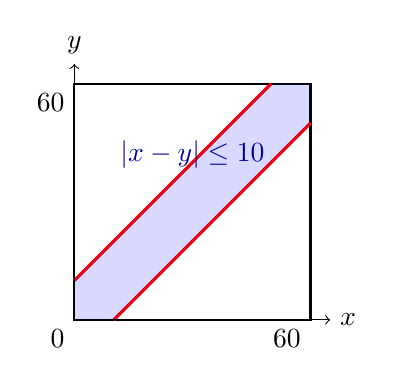
\begin{tikzpicture}[scale=0.05]
            % 绘制正方形区域
            \draw[thick] (0,0) rectangle (60,60);
            % 绘制两条界限直线: x-y=10  与 x-y=-10
            \draw[red,very thick] (10,0) -- (60,50);   % x - y = 10
            \draw[red,very thick] (0,10) -- (50,60);   % x - y = -10
            % 填充有效区域
            \fill[blue,opacity=0.15] 
                (0,10) -- (10,0) -- (60,50) -- (50,60) -- cycle;
            % 漏画了两个小的角
            \fill[blue,opacity=0.15]
                (0,0) -- (0,10) -- (10,0) -- cycle;
            \fill[blue,opacity=0.15]
                (60,60) -- (60,50) -- (50,60) -- cycle;
            % 坐标轴
            \draw[->] (0,0) -- (65,0) node[right] {$x$};
            \draw[->] (0,0) -- (0,65) node[above] {$y$};
            % 标注几个重要点
            \foreach \p/\lab in {(0,0)/0, (60,0)/60, (0,60)/60} {
                \draw \p node[below left]{\lab};
            }
            % 标签
            \node[blue!60!black] at (30,42) {$|x-y|\leq 10$};
        \end{tikzpicture}
        \end{center}
        因而概率是
        \[
        \mathbb{P}(E) = \frac{m(E)}{m(\Omega)} = \frac{3600-2500}{3600} = \frac{11}{36}
        \]
    \end{solution}
\end{example}



\section{conditional probability}
\begin{definition}{conditional probability}
    对于 probability space \((\Omega, \mathcal{F}, \mathbb{P})\), 给定一个 event $B \in \mathcal{F}$, 如果 \(\mathbb{P}(B) > 0\), 我们定义 conditional probability of an event $A \in \mathcal{F}$ given $B$ 为:
    \[
    \mathbb{P}(A \mid B) = \frac{\mathbb{P}(A \cap B)}{\mathbb{P}(B)}
    \]
\end{definition}
\begin{proposition}{decomposing probability of intersection of events}   
    令 $\left(A_i\right)_{i \in \mathbb{N}}$ 为一个 seq of events, 对于任意 $n \in \mathbb{N}$:
    \[
    \mathbb{P}\left(A_1 \cap A_2 \cap \ldots \cap A_n\right)=\mathbb{P}\left(A_1\right) \cdot \mathbb{P}\left(A_2 \mid A_1\right) \cdot \mathbb{P}\left(A_3 \mid A_1 \cap A_2\right) \ldots \cdot \mathbb{P}\left(A_n \mid A_1 \cap \ldots \cap A_{n-1}\right)
    \]
\end{proposition}
\begin{proof}
Naturally follows from the def. 
\end{proof}


\subsection{Law of total probability and Bayes' Theorem}
\begin{theorem}{law of total probability}
    令 $\left(A_i\right)_{i \in \mathbb{N}}$ 为一个 seq of \textbf{pairwise disjoint} events, 如果 $\sqcup_{i=1}^{\infty} A_i=\Omega$, 那么对于任意 event $E \subseteq \Omega$:
    \[
    \mathbb{P}(E)=\sum_{i=1}^{\infty} \mathbb{P}\left(A_i\right) \mathbb{P}\left(E \mid A_i\right)
    \]
\end{theorem}
\begin{proof}
    \[
    \mathbb{P}(E)=\mathbb{P}\left(E \cap \cup_{i=1}^{\infty} A_i\right)=\mathbb{P}\left(\cup_{i=1}^{\infty} E \cap A_i\right)=\sum_{i=1}^{\infty} \mathbb{P}\left(E \cap A_i\right)=\sum_{i=1}^{\infty} \mathbb{P}\left(A_i\right) \mathbb{P}\left(E \mid A_i\right)
    \]
\end{proof}
\begin{remark}
    \(P(A_i)P(E\mid A_i)\) 就等于 \(P(E \cap A_i)\), 也就是在 \(A_i\) 这个区域上, \(E\) 的 measure. 因而 disjoint union 之下就是 \(E\) 的完整 measure.
\end{remark}

\begin{theorem}{Bayes theorem}
    If $A, B \subseteq \Omega$ such that $\mathbb{P}(B) \neq 0$, then
    \[
    \mathbb{P}(A \mid B)=\frac{\mathbb{P}(A) \cdot \mathbb{P}(B \mid A)}{\mathbb{P}(B)}
    \]
\end{theorem}
\begin{remark}
    这其实是一个非常直接的结果, 因为 \(P(A) \dot P(B \mid A) = P(A \cap B)\). \\
    但是它的意义在于, 如果我们知道两个事件的概率和其中一个对另一个的条件概率, 我们就也得到了反过来的条件概率.
\end{remark}



\begin{example}{(Medical testing)}

在一个群体中, 随机选取一个人患有某种罕见疾病的概率是 0.001. 该疾病有一个诊断测试, 其性质如下: 给定个体患病, 测试呈阳性的概率 (真正阳性率) 是 0.99. 给定个体健康, 测试呈阳性的概率 (假阳性率) 是 0.02. 从群体中随机选取的一个人测试呈阳性. 该个体实际上患有该疾病的概率是多少?
于是
\begin{solution}
由 law of total probability, 我们有
\[
 \mathbb{P}(\text {positive})= \mathbb{P}(\text{positive} \mid \text{sick}) \mathbb{P}(\text{sick}) + \mathbb{P}(\text{positive} \mid \text{healthy}) \mathbb{P}(\text{healthy}) = 0.99 \cdot 0.001 + 0.02 \cdot 0.999 = 0.02097
\]
于是
\[
\mathbb{P}(\text {sick} \mid \text {positive})=\frac{0.99 \cdot 0.001}{0.02097} \approx 0.047
\]
\end{solution}
\end{example}

\begin{example}{(Monty Hall problem)}

假设你参加一个游戏节目, 面前有三扇门: 一扇门后面有一辆车; 其他两扇门后面是山羊. 你选择了一扇门, 比如说是 1 号门, 然后主持人打开了另一扇门, 比如说是 3 号门, 里面有一只山羊. 然后他说 "你想换成 2 号门吗?". 换门对你有利吗?
\begin{solution}
令 \(A_i\) 表示: car 在 \(i\) 号门后面; \(B\) 事件表示: 主持人打开 3 号门. 我们要求的概率是在事件 \(B\) 发生的情况下, \(A_2\) 的个概率, 即 \(\mathbb{P}(A_2 \mid B)\). 它的大小是:
\begin{align*}
\mathbb{P}(A_2 \mid B) &= \frac{\mathbb{P}(A_2) \cdot \mathbb{P}(B \mid A_2)}{\mathbb{P}(B)} \\
&= \frac{\mathbb{P}(B \mid A_2)\mathbb{P}(A_2)}{\mathbb{P}(B\mid A_1)\mathbb{P}(A_1) + \mathbb{P}(B\mid A_2)\mathbb{P}(A_2) + \mathbb{P}(B\mid A_3)\mathbb{P}(A_3)}    \\
&= \frac{1 \cdot \frac{1}{3}}{\frac{1}{2} \cdot \frac{1}{3} + 1 \cdot \frac{1}{3} + 0 \cdot \frac{1}{3}} = \frac{2}{3} > \frac{1}{3}
\end{align*}
因而, 换门是有利的.
\end{solution}
\begin{remark}
这是一个非常反直觉的例子. 我们直觉肯定会觉得: 一共 1 辆车和 2 个山羊, 主持人帮忙排除掉了一个山羊, 
那么剩下来的两个里面我们二选一, 肯定是 $1/2$ 概率, 而这个 "更换与否" 就是二选一的抉择. 但其实不是这样的. \\
在第一次选择和第二次选择之间, 主持人带来了额外的信息. 
\begin{itemize}
    \item 不换门: win iff 在一开始就选择对了车, 这个概率是 $1/3$.
    \item 换门: win iff 在一开始选择的是山羊, 这个概率是 $2/3$.
\end{itemize}
从条件概率的视角来看: 
\begin{itemize}
    \item 如果车在 2 号门: 主持人在这个环节里只能选择 3 号门.
    \item 如果车在 1 号门: 主持人在这个环节里可以随机在 2 号和 3 号门里面选择一扇门.
\end{itemize}
也就是说, 主持人打开 3 号门的这个动作, 把 3 号门原本含有的 "中奖潜力" 全部转移给了 2 号门.
这很反直觉. 但是可以用一段 python 程序验证:

\begin{python}[caption={Monty Hall problem simulation}, label=code:montyhall-sim]
import random

def monty_hall_sim(trials=10000):
    stay_wins = 0
    switch_wins = 0

    for _ in range(trials):
        # 1. 初始化门: 0代表羊, 1代表车
        doors = [0, 0, 0]
        car_position = random.randint(0, 2)
        doors[car_position] = 1
        
        # 2. 玩家最初的选择
        player_choice = random.randint(0, 2)
        
        # 3. 主持人打开一扇有山羊的门
        # 主持人不能开玩家选的门,也不能开有车的门
        possible_host_doors = [
            i for i in range(3) 
            if i != player_choice and doors[i] == 0
        ]
        host_opens = random.choice(possible_host_doors)
        
        # 4. 如果"坚持不换"赢了
        if doors[player_choice] == 1:
            stay_wins += 1
            
        # 5. 如果"换门"赢了
        # 换门后的选择是:既不是原选,也不是主持人开的那扇
        remaining_door = [
            i for i in range(3) 
            if i != player_choice and i != host_opens
        ][0]
        
        if doors[remaining_door] == 1:
            switch_wins += 1

    print(f"总实验次数: {trials}")
    print(f"坚持不换中奖次数: {stay_wins} (概率: {stay_wins/trials:.2%})")
    print(f"换门后中奖次数: {switch_wins} (概率: {switch_wins/trials:.2%})")

if __name__ == "__main__":
    monty_hall_sim()
\end{python}
运行结果:

\begin{terminal}[caption={Monty Hall problem simulation result}]
总实验次数: 10000  
坚持不换中奖次数: 3312 (概率: 33.12%)
换门后中奖次数: 6688 (概率: 66.88%) 
\end{terminal}
\end{remark}
\end{example}



\begin{example}{(Wizards)}

两个巫师 \(A\) 和 \(B\) 进行决斗, 他们轮流射击对方. 巫师 \(A\) 每次射击命中 \(B\) 的概率是 \(\mathbb{P}(A)=\frac{1}{2}\), 而巫师 \(B\) 每次射击命中 \(A\) 的概率是 \(\mathbb{P}(B)=\frac{2}{3}\). 巫师 \(A\) 先开枪. 求: 巫师 \(A\) 获胜的概率是多少? \\
\begin{solution}
任意一轮射击 (假设前一轮没有结束, 于是游戏回到初始状态. 因而任意一轮都是独立的) 中,
令 \(W_A\) 为事件: \(A\) 获胜; \(W_B\) 为事件: \(B\) 获胜, 假设他们从各自开始射击. 根据全概率公式, 我们有
$$
\begin{aligned}
& \mathbb{P}\left(W_A\right)=\mathbb{P}(\mathrm{hit}) \mathbb{P}\left(W_A \mid \mathrm{hit}\right)+\mathbb{P}(\mathrm{miss}) \mathbb{P}\left(W_A \mid \mathrm{miss}\right)=\frac{1}{2}+\frac{1}{2} \mathbb{P}\left(W_B^c\right) \\
& \mathbb{P}\left(W_B\right)=\mathbb{P}(\mathrm{hit}) \mathbb{P}\left(W_B \mid \mathrm{hit}\right)+\mathbb{P}(\mathrm{miss}) \mathbb{P}\left(W_B \mid \mathrm{miss}\right)=\frac{2}{3}+\frac{1}{3} \mathbb{P}\left(W_A^c\right)
\end{aligned}
$$
Solving the system, we find $\mathbb{P}\left(W_A\right)=0.6$.
\end{solution}
\begin{remark}
这个例子表明了先手优势有多大. 相比上一个例子, 这是很直观的.\\
另外, 这个例子有趣的是, 我们把无限的回合转化为了一个循环结构, 利用游戏状态的自相似, 只需要考虑任意一轮即可.
\end{remark}    
\end{example}

\subsection{Kolmogorov definition of conditional probability}
我们通过 \(\mathbb{P}(A \mid B) = \frac{\mathbb{P}(A \cap B)}{\mathbb{P}(B)}\) 定义出来的 conditional probability 有一个限制, 就是 enforce \(\mathbb{P}(B) > 0\). \\
但是, 难道 \(\mathbb{P}(B) = 0\) 就不能定义条件概率了吗? 我们考虑一个连续情况: 在 \(\mathbb{R}^3\) 中任意选择一个点, 求: 该点位于单位球面上的概率. 显然, 这个概率是 0. 但是, 如果我们知道该点位于单位球内, 那么该点距离原点的距离为 \(1\) 的概率应当为 \(1\). 也就是说,  即使在 \(\mathbb{P}(B) = 0\) 的情况下, 我们也希望定义 \(\mathbb{P}(A \mid B)\).\\
在考虑这个定义之前, 首先我们发现: 基于我们先前定义的 conditional probability, 我们可以获得一个新的 probability space:
\begin{definition}{conditional probability space and trace $\sigma$-algebra}
    对于给定的 prob space \((\Omega, \mathcal{F}, \mathbb{P})\), 给定一个 event \(B \in \mathcal{F}\) 且 \(\mathbb{P}(B) > 0\), 我们定义 conditional probability space as the triplet \((B, \mathcal{F}_B, \mathbb{P}(\cdot \mid B))\), 其中:
    \[
    F_B := \{A\cap B \mid  A \in \mathcal{F} \}
    \]
    被称为 \textbf{trace \(\sigma\)-algebra on \(B\)}.\\
    容易验证, 这个 triplet 是一个 prob space.
\end{definition}
\begin{remark}
    当我们把整个 prob space 限制在 event \(B\) 上时, 本质上是在做一个 Radon-Nikodym derivative 的操作.\\
    定义 \(f:= \frac{\mathbb{I}_B}{\mathbb{P}(B)}\), 那么对于任意 event \(A \in \mathcal{F_B}\), 有:
    \[
    \mathbb{P}(A \mid B) = \int_{A} f \, d\mathbb{P}
    \] 
    因而和我们的直觉一样, 条件概率是通过一个 density function 来重新加权原本的概率测度. 
\end{remark}
既然这样, 我们能否直接从一个新的 prob space \((B, \mathcal{F}_B, \mathbb{P}(\cdot \mid B))\) 出发, 来定义条件概率呢? 这就是 Kolmogorov 的定义:
\begin{definition}{Kolmogorov definition of conditional probability}
    对于给定的 prob space \((\Omega, \mathcal{F}, \mathbb{P})\), 
    设 \(\mathcal{G} \subseteq \mathcal{F}\) 是一个 sub-\(\sigma\)-algebra. 对于 event \(A \in \mathcal{F}\), 条件概率 \(\mathbb{P}(A \mid \mathcal{G})\) 是一个 \(\mathcal{G}\)-measurable 的随机变量, 其满足对于任意 \(G \in \mathcal{G}\), 有:
    \[
    \int_G \mathbb{P} (A \mid \mathcal{G}) \, d\mathbb{P} = \mathbb{P}(A \cap G)
    \]
    显然, 当 \(\mathbb{P}(B) > 0\) 时, 这个定义和我们之前的定义是等价的.\\
    这个 random variable \(\mathbb{P}(A \mid \mathcal{G})\) 在 \(\mathbb{P}\)-a.s. 意义下是唯一的.
\end{definition}
\begin{remark}
    条件概率 \(\mathbb{P}(A \mid \mathcal{G})\) 这个测度是 \(\mathbb{P}(A \cap \cdot)\) 这个测度相对于背景测度 \(\mathbb{P}\) 在子信息流 \(\mathcal{G}\) 下的 Radon-Nikodym derivative, 也就是一个密度函数. \\
    这个定义里没有指明, 给定一个 event \(B \in \mathcal{F}\), 如何去确定 \(\mathcal{G}\) 以及 \(\mathbb{P}(A \mid \mathcal{G})\). 虽然这是一个抽象的存在性 \(\&\) 唯一性定义, 但是标准的做法是:
    \begin{itemize}
        \item  看向产生 \(B\) 的 random variable \(X\), 即 \(B = \{X = x\}\), 令 \(\mathcal{G} = \sigma(X)\), 即由 random variable \(X\) 生成的 \(\sigma\)-algebra. 这个 \(\sigma\)-algebra 包含了所有关于 \(X\) 可能取值的信息.
        \item 既然 $\mathbb{P}(A \mid \sigma(X))$ 是关于 $\sigma(X)$ 可测的, 那么它一定可以写成 $h(X)$ 的形式. 通过对 $X$ 的所有可能取值进行积分, 我们确定了函数 $h(\cdot)$ 的整体形态, 这时我们定义 $P(A \mid X=x)$ 为函数 $h$ 在点 $x$ 处的值.
        \item \(\mathbb{P}(A \mid \mathcal{G})\) 实际就是条件期望 \(\mathbb{E}[\mathbb{I}_A \mid \mathcal{G}]\). 当 \(\mathbb{P}(B) > 0\) 时, 它就退化回经典定义 \( \frac{\mathbb{P}(A \cap B)}{\mathbb{P}(B)}\).
    \end{itemize}
\end{remark}
\begin{remark}
    Further issue: \textbf{Borel-Kolmogorov paradox}.\\
    即便是这个定义, 也会出现问题. \\
    给定一个事件 $B$, 如果 $\mathbb{P}(B)=0$, 则 $\mathbb{P}(A \mid B)$ 的取值取决于我们将 $B$ 嵌入到哪一个随机变量 $X$ 中.
不同的随机变量 $X, Y$ 即使都能产生相同的事件 $\{X=x\} = \{Y=y\} = B$, 它们生成的子 $\sigma$-代数 $\sigma(X)$ 和 $\sigma(Y)$ 却不同, 导致最终确定的条件概率 $h_X(x) \neq h_Y(y)$. \\
为了解决这个问题, 可以引入更精细的结构, 比如说 regular conditional probability, 以及 disintegration theorem. 不过此处不展开了.
\end{remark}

\section{independence}
\begin{definition}{independence of events}
    对于 prob space \((\Omega, \mathcal{F}, \mathbb{P})\), 两个 events \(A, B \in \mathcal{F}\) 如果有
    \[
    \mathbb{P}(A \cap B) = \mathbb{P}(A) \cdot \mathbb{P}(B)
    \]
    则称 \(A\) 和 \(B\) 是 independent 的.\\
    更加 generally, 对于任意 collection of events \(\{A_i\}_{i \in I}\), 如果对于任意有限子集 \(J \subseteq I\), 有 
    \[
    \mathbb{P}\left(\bigcap_{j \in J} A_j\right) = \prod_{j \in J} \mathbb{P}(A_j)
    \]
    则称 \(\{A_i\}_{i \in I}\) 是 mutually independent 的.
\end{definition}
\begin{remark}
    根据条件概率的定义, 容易得出: 两个 events \(A, B\) independent 的定义\textbf{等价于 \(\mathbb{P}(A \mid B) = \mathbb{P}(A)\)}, 即事件 \(B\) 的发生与否不影响事件 \(A\) 发生的概率.\\
    将它推广到多个事件: 即\textbf{任意一个事件的发生与否都不影响其他事件发生的概率}.
\end{remark}

\begin{proposition}
    如果 events \(A\) 和 \(B\) independent, 则 \(A\) 和 \(B^c\) 也是 independent 的.
\end{proposition}
\begin{proof}
\[
\begin{aligned}
\mathbb{P}\left(A^c \cap B^c\right) & =\mathbb{P}\left((A \cup B)^c\right)=1-\mathbb{P}(A \cup B)=1-\mathbb{P}(A)-\mathbb{P}(B)+\mathbb{P}(A \cap B) \\
& =1-\mathbb{P}(A)-\mathbb{P}(B)+\mathbb{P}(A) \cdot \mathbb{P}(B) = (1-\mathbb{P}(A))(1-\mathbb{P}(B)) \\
& =\mathbb{P}\left(A^c\right) \cdot \mathbb{P}\left(B^c\right)
\end{aligned}
\]
\end{proof}


\begin{example}{(Pairwise Independence vs. Mutual Independence)}

一组事件 $A_1, A_2, \ldots \in \mathcal{F}$ 如果是 mutually independent 的, 则它们两两 independent. \textbf{但是反过来不成立}.\\
即: \textbf{即便对于任意 $i \neq j$, 有 $\mathbb{P}(A_i \cap A_j) = \mathbb{P}(A_i) \mathbb{P}(A_j)$, 也并不意味着这些事件是 mutually independent 的}.\\
下面为一个 counterexample: 考虑掷两个骰子. 令事件
$$
A:=\{\text{first roll is } 4\}, \quad B:=\{\text{second roll is } 3\},\quad C:=\{\text{the sum of the two outcomes is } 7\}
$$
我们发现: $\mathbb{P}(A \cap B \cap C)=\frac{1}{36} \neq \mathbb{P}(A) \mathbb{P}(B) \mathbb{P}(C)=\frac{1}{6^3}$, 因而 $A, B, C$ 并不 mutually independent. 然而, However, $\mathbb{P}(A \cap B)=\frac{1}{36}=\mathbb{P}(A) \mathbb{P}(B), \mathbb{P}(A \cap C)=\frac{1}{36}=\mathbb{P}(A) \mathbb{P}(C)$ and $\mathbb{P}(B \cap C)=\frac{1}{36}=\mathbb{P}(B) \mathbb{P}(C)$, 
因而它们两两 pairwise independent.
\end{example}
\begin{remark}
这个反例能够成功的理由是: 事件 $C$ (总和) 和 事件 $A$ (第一个骰子) 以及事件 $B$ (第二个骰子) 分别都是独立的, 因为知道了其中一个并不会影响另一个的概率. 但是, 一旦我们知道了 $A$ 和 $B$ 的值, 那么 $C$ 的值就被完全确定了 (因为总和就是两个骰子的和). 因而, 三个事件并不 mutually independent. \\
(注意: 如果 \(C\) 事件不是和为 7 而是一个小于 7 的数, 那就不是了, 因为如果我们知道第一次是 6, 那么和就不可能是 6, 那么就也失去了 pairwise independence).\\
这个例子说明了, mutual independence 是一个比较强的条件.
我们可以把这三个事件看作是对结果空间的约束:
\begin{itemize}
    \item 两个骰子的结果空间有 36 个点.
    \item $A$ 是一条线 (6个点), $B$ 是另一条线 (6个点), $C$ 是一条对角线 (6个点)。
    \item 两两独立: 意味着任意两条线相交的点数, 恰好符合概率乘积.
    \item 相互独立: 要求这三条线交于一点的概率也符合乘积. 
\end{itemize}
这个例子提醒我们: 独立性不是一种可以由低维向高维简单“归纳”的性质. 一个系统可以局部解耦(两两独立, 但在全局尺度上却存在强耦合. 总之 mutual independence 是一个很强的条件.
\end{remark}



\begin{example}{(coin tossing)}

假设我们有一枚不均匀的硬币, 掷出正面的概率是 $p \in[0,1]$, 反面的概率是 $1-p$. 我们不断地掷这枚硬币, 直到第一次掷出正面为止, 并记录所需的掷币次数. 求: 掷币次数为奇数的概率是多少?
\begin{solution}
对于任意 $i \in \mathbb{N}$, 考虑事件 $A_i=\{$ 掷币次数为 $i\}$.
$$
\mathbb{P}\left(\cup_{n=1}^{\infty} A_{2 n-1}\right)=\sum_{n=1}^{\infty} \mathbb{P}\left(A_{2 n-1}\right)=\sum_{n=1}^{\infty}(1-p)^{2 n-2} p=p \sum_{n=1}^{\infty}\left((1-p)^2\right)^{n-1}=p \cdot \frac{1}{1-(1-p)^2}=\frac{1}{2-p}
$$
\end{solution}
\begin{remark}
这个问题还可以通过 law of total probability 来解决.\\
令 $E=$ 掷币次数为奇数. 那么
$$
\begin{aligned}
\mathbb{P}(E) & =\mathbb{P}(\text{head}) \cdot \mathbb{P}(E \mid \text{head})+\mathbb{P}(\text{tail}) \cdot \mathbb{P}(E \mid \text{tail}) \\
& =p \cdot 1+(1-p) \cdot(1-\mathbb{P}(E))
\end{aligned}
$$
Solve 这个 equation 得到同样结果.
\end{remark}    
\end{example}